% -------------------------------------------------------------------------
%  MusicFormats Library
%  Copyright (C) Jacques Menu 2016-2023

%  This Source Code Form is subject to the terms of the Mozilla Public
%  License, v. 2.0. If a copy of the MPL was not distributed with this
%  file, you can obtain one at http://mozilla.org/MPL/2.0/.

%  https://github.com/jacques-menu/musicformats
% -------------------------------------------------------------------------

\documentclass[12pt,a4paper]{article}


% -------------------------------------------------------------------------
% import common LaTeX settings
% -------------------------------------------------------------------------

\usepackage{import}

\subimport{../CommonLaTeXFiles}{CommonSettings.tex}

\subimport{../CommonLaTeXFiles}{Indexing.tex}

\subimport{../CommonLaTeXFiles}{FontsAndColors.tex}

\subimport{../CommonLaTeXFiles}{Referencing.tex}

\subimport{../CommonLaTeXFiles}{MusicFormatsNames.tex}

\subimport{../CommonLaTeXFiles}{MusicFormatsCommands.tex}

\subimport{../CommonLaTeXFiles}{MusicFormatsFilesAndFolders.tex}

\subimport{../CommonLaTeXFiles}{Shortcuts.tex}

\subimport{../CommonLaTeXFiles}{Listings.tex}


% -------------------------------------------------------------------------
\begin{document}
% -------------------------------------------------------------------------

% defeat headwidth not being equal to \textwidth %%%JMI should not be necessary ???
\setlength{\headwidth}{\textwidth}


%% use the first page fancyhead headers and footers
\useFirstPageHeadersAndFooters


%\noindent

\title{
Introduction to \mxml\\[5pt]
%\large {Notensatz-Konferenz, Salzburg Mozarteum, January 17-18, 2020}
}

\newsavebox{\authorBox}
\sbox{\authorBox}{
\raisebox{-0.35em}{
\begin{minipage}{\textwidth}
\footnotesize%
Former lecturer in computer science at Centre Universitaire d'Informatique,\\
University of Geneva, Switzerland
\end{minipage}
}
}

\author{
Jacques Menu
%\footnote{
%\usebox{\authorBox}
%}
}

\newcommand{\revision}{revision 1.2}

\date {\normalsize \today, \revision}
%\date {}

\maketitle

%\thispagestyle{fancy} % right after \maketitle to apply it to the first page too

% use the first page fancyhead headers and footers
%\useListsPagesHeadersAndFooters


\abstract {
This document presents a basic view of \mxml\ and a couple of short examples illustrating how \mxml\ represents a music score. Our goal is to give a flavor of what \mxml\ definitions and data look like from a musician's point of view. We use a combination of formal definitions from the \mxml\ DTD and free text explanations.

\sep

All the examples mentioned can be downloaded from \url{https://github.com/jacques-menu/musicformats/tree/master/musicxml}. They are grouped by subject in subdirectories, such as \gitmxmlfile{basic/HelloWorld.xml}.

\sep

The contents of this document is verbose... because \mxml\ itself is!
}

{ % reduce vertical size of tables and lists
	\small

  \setlength {\parskip} {0.25ex plus \baselineskip minus 2pt}

% use the lists fancyhead headers and footers
%\useListsPagesHeadersAndFooters

	\tableofcontents

	%\listoffigures

	\lstlistoflistings
}


% -------------------------------------------------------------------------
% -------------------------------------------------------------------------
\section{Software tools used}
% -------------------------------------------------------------------------
% -------------------------------------------------------------------------

\mxml\ files have been named with a '\fileName{\tt .xml}' suffix for years, until it was decided rather recently that this should be changed to '{\tt .musicxml}'. There are GUI applications that filter the file names in their '{\tt open}' or '{\tt import}' dialogs and don't know that change yet, though. We will thus stick to the '\fileName{\tt .xml}' suffix convention.

\sep

The scores fragments shown in this document have been produced by translating the '\fileName{\tt .xml}' file to LilyPond\ syntax, and then creating the graphical score with \lily.

\sep

The translations have been done by \xmlToLy, a prototype tool developed by this author. \xmlToLy\ and some of the specific examples presented in this document are this author's contribution to \libmusicxml, an open-source C++ library created and maintained by \fober at Grame, Lyon, France.

The home page to \libmusicxml\ is \url{https://github.com/jacques-menu/musicformats}, and \xmlToLy\ is in the '\fileName{\tt lilypond}' \branch.

\sep

The reader is invited to handle the '\fileName{\tt .xml}' file examples with their own software tools to compare the results with the ones herein.

\sep

Other score editing applications are mentioned in this document, namely \sib,
\fin\ and \muse\ (\url{https://musescore.org}), which is open-source.
This author doesn't own licenses for other commercial applications such as Dorico\texttrademark\ or Capella\texttrademark.

\sep

\mxmlToLy\ is mentioned too: this \converter\ of \mxml\ to \lily\ is supplied with \lily. The design goals of \xmlToLy\ are to perform at least as well as \mxmlToLy, while providing as many options as needed to avoid too much editing of the \lcg.

\sep \sep


% -------------------------------------------------------------------------
% -------------------------------------------------------------------------
\section{Overview of MusicXML}
% -------------------------------------------------------------------------
% -------------------------------------------------------------------------


% now we can switch to the regular headers and footers
\useRegularPagesHeadersAndFooters


% -------------------------------------------------------------------------
\subsection{What is MusicXML?}
% -------------------------------------------------------------------------

\mxml\ (\MainIt{Music eXtended Markup Language}, \url{https://www.musicxml.com}) is a specification language meant to represent western notation music scores by texts, readable both by humans and computers, and to help sharing music score files between applications, through export and import mechanisms..

It has been invented by Michael Good and initially developed by Recordare LLC, which was bought by MakeMusic in 2011, and finally transferred to the W3C Music Notation Community Group (\url{https://www.w3.org/community/music-notation/}) in 2015. See \url{https://en.wikipedia.org/wiki/MusicXML} for more historical details.

\sep

\mxml\ data contains very detailed information about the music score, and it is \MainIt{quite verbose} by nature. This makes creating such data by hand very difficult, and this is done by applications actually.


% -------------------------------------------------------------------------
\subsection{Part-wise vs. measure-wise descriptions}
% -------------------------------------------------------------------------

\mxml\ allows the score to be represented as a sequence of parts, each containing a sequence of measures, or as a sequence of measures, each containing a sequence of parts, i.e. data describing the contents of the corresponding measure in a part.

\sep

It seems that measure-wise descriptions have been very little used and then abandoned, and we shall stick to part-wise \mxml\ data in this document.

As a historical note, an XSL/XSLT script was supplied in the early days of \mxml\ to convert between part-wise and measure-wise formats.


% -------------------------------------------------------------------------
\subsection{MusicXML's formal definition}
\mylabel{formalDefinition}
% -------------------------------------------------------------------------

As a member of the *XML family of languages, \mxml\ is defined by a DTD (\MainIt{Document Type Definition}), to be found at \url{https://github.com/w3c/musicxml/tree/v3.1}.

\sep

An *XML DTD defines:
\begin{itemize}
\item \MainIt{elements}, used to structure the data since they can be nested;
\item \MainIt{attributes}, that attach named values to the elements;
\item \MainIt{entities}, which are names of groups of elements, such as '{\tt layout-tenths}' and '{\tt start-stop}'. There are used to structure the DTD itself when those elements occur at multiple places in the DTD, and make the latter more readable and easier to update.
\end{itemize}

\sep

For example, consider:
\begin{lstlisting}[language=MusicXML]
  <part id="P1">
    <measure number="1" width="464.29">
		<!-- ... ... ... ... ... -->
\end{lstlisting}

We see that:
\begin{itemize}
\item the \musicXmlMarkup{part} element contains a nested \musicXmlMarkup{measure} element;
\item the \musicXmlMarkup{part} element has an '\musicXmlAttribute{id}' attribute containing the name of the part, '\musicXmlAttribute{P1}';%%%JMI
\item the \musicXmlMarkup{measure} element's attributes contain measure number '{\tt 1}'and width '{\tt 464.29}'.
\end{itemize}

Some elements contain a single unnamed data item, such as durations and voice and staff numbers:
\begin{lstlisting}[language=MusicXML]
        <duration>4</duration>
        <voice>2</voice>
        <staff>1</staff>
\end{lstlisting}

\sep

The \gitsubdir{dtds/3.1/schema} subdirectory contains '\fileName{\tt *.mod}' text files defining the various concepts. The file \gitschemafile{common.mod} contains definitions used in other '\fileName{\tt *.mod}' files:
\begin{lstlisting}[language=MusicXML]
<!--
	This file contains entities and elements that are common
	across multiple DTD modules. In particular, several elements
	here are common across both notes and measures.
-->
\end{lstlisting}

\sep

For example, \gitschemafile{note.mod} defines the \musicXmlMarkup{backup} and \musicXmlMarkup{forward} markups this way:
\begin{lstlisting}[language=MusicXML, caption={{\tt <backup/>} and {\tt <forward/>} definition}]
<!--
	The backup and forward elements are required to coordinate
	multiple voices in one part, including music on multiple
	staves. The forward element is generally used within voices
	and staves, while the backup element is generally used to
	move between voices and staves. Thus the backup element
	does not include voice or staff elements. NotesDuration values
	should always be positive, and should not cross measure
	boundaries or mid-measure changes in the divisions value.
-->
<!ELEMENT backup (duration, %editorial;)>
<!ELEMENT forward
	(duration, %editorial-voice;, staff?)>
\end{lstlisting}

An example of their use is:
\begin{lstlisting}[language=MusicXML, caption={{\tt <backup/>} and {\tt <forward/>} example}]
      <forward>
        <duration>4</duration>
        <voice>2</voice>
        <staff>1</staff>
      </forward>
      <backup>
        <duration>8</duration>
      </backup>
\end{lstlisting}

\sep

In DTDs, sub-elements can be followed by one of these characters, which mean, as is usual in computer science:
\begin{itemize}
\item'{\tt ?}': 0 or 1 occurence, i.e. optional;
\item'{\tt *}': 0 or more occurrences;
\item'{\tt +}': 1 or more occurrences.
\end{itemize}

One can see in the definition of the '\musicXmlMarkup{<forward>}' element that the '\musicXmlMarkup{<duration>}' element is mandatory, while the '\musicXmlMarkup{<staff>}' element is optional. The text in the DTD tells that staff 1 in implied if it not specified.

\sep

In a DTD, '\musicXmlMarkup{CDATA}' means \MainIt{Character Data}. Such data is not analyzed by the software  that reads the \mxml\ data, it is merely passed over verbatim to whoever asked the data to be read in.

In the same vein, '\musicXmlMarkup{PCDATA}' means \MainIt{Parsed Character Data}, that is, mixed content XML data that are analyzed by software tools.

\sep

The current version of the \mxml\ DTD is~3.1, and there are discussions about version~3.2.

\sep

The syntactical aspects of \mxml\ are quite simple and regular, which makes it easy to handle \mxml\ data with algorithms.

\page


% -------------------------------------------------------------------------
\subsection{Markups}
% -------------------------------------------------------------------------

\mxml\ data is made of so-called markups (the 'M' in 'XML'), delimited by an \MainIt{start-tag} and a \MainIt{stop-tag}.

The start-tag is introduced by a '{\tt <}' and closed by a '{\tt >}', as in '\musicXmlMarkup{<part-list>}'. The stop-tag is introduced by a '{\tt </}' and closed by a '{\tt >}', as in '\musicXmlMarkup{</part-list>}'.

\sep

Markups go by pairs, as in:
\begin{lstlisting}[language=MusicXML]
        <duration>4</duration>
\end{lstlisting}

The spaces and end of lines between markups are ignored.

\sep

It is possible to contract an element that contains nothing between its start-tag and stop-tag, such as:
\begin{lstlisting}[language=MusicXML]
        <dot></dot>
\end{lstlisting}
which can be written:
\begin{lstlisting}[language=MusicXML]
        <dot />
\end{lstlisting}

\sep

We shall call \MainIt{sub-element} and element nested into another one. '\musicXmlMarkup{<part-name>}' is thus a sub-element of element '\musicXmlMarkup{<score-part}' above.

\sep

The values of attributes can be double-quoted characters strings and integer or floating point numbers.

Some attributes are mandatory such as '{\tt id}' in '{\tt <score-part>}', while others are optional.

\sep

Comments can be used in \mxml\ data. They start with a '{\tt <!--}' start-tag and end with a '{\tt -->}' stop-tag, as in:
\begin{lstlisting}[language=MusicXML]
<!--=========================================================-->
    <measure number="1">
  <!-- A very minimal MusicXML example, part P1, measure 1 -->
\end{lstlisting}

Comments can span several lines.

\sep

\hand {\mxml\ is a representation of HOW TO DRAW a score, which has implications on the kind of markups available, in particular '{\tt <forward>}' and '{\tt <backup>}', which are presented at \mylink{multipleVoices}.
}

The syntax of \mxml\ data quite regular and simple, and it is easy to program lexical/syntactical analyzers for it.


% -------------------------------------------------------------------------
\subsection{Overall structure of MusicXML data}
% -------------------------------------------------------------------------

\mxml\ data consists of:
\begin{itemize}
\item a '{\tt <?xml>}' element indicating the characters encoding used;
\item a '{\tt <!DOCTYPE>}' element telling that the contents is in '{\tt score-partwise}' mode;
\item a '{\tt <score-partwise>}' element indicating the \mxml\ DTD number that the forthcoming data complies to, and that contains:

\item a score header containing:

\begin{itemize}
  \item an optional '{\tt <work>}' element, containing sub-elements such as '{\tt <work-number>}', \\
  '{\tt <work-title>}' and '{\tt <opus>}';

  \item optional '{\tt <movement-number>}', '{\tt <movement-title>}', '{\tt <identification>}' and \\
  '{\tt <defaults>}' sub-elements;

  \item 0 or more '{\tt <credit>}' elements;

  \item a '{\tt <part-list>}' element containing the various '{\tt <score-part>}'s in the score;
  \end{itemize}

\item a sequence of '{\tt <part>}' elements in the order they appear in the score, each one containing the measures in the given part, in order.
\end{itemize}

Here is how the score header is actually defined in \gitschemafile{score.mod}:
\begin{lstlisting}[language=MusicXML]
<!--
	The score-header entity contains basic score metadata
	about the work and movement, score-wide defaults for
	layout and fonts, credits that appear on the first page,
	and the part list.
-->
<!ENTITY % score-header
	"(work?, movement-number?, movement-title?,
	  identification?, defaults?, credit*, part-list)">
\end{lstlisting}


% -------------------------------------------------------------------------
\subsection{What is the semantics of MusicXML data?}
% -------------------------------------------------------------------------

We have seen in section \mylink{formalDefinition}, that not specifying the staff number in a '{\tt <forward>}' element implies a value of one.

It is very difficult to define the semantics -- the meaning of the sentences -- of an artificial language in a complete and consistent way, i.e. without omitting anything and without contradictions.

\mxml\ is no std::exception to this rule: there are things unsaid in the DTD, which leaves room to interpretation by the various applications that create or handle \mxml\ data.

\sep

For example, clefs are defined in \gitschemafile{attributes.mod}, starting with:
\begin{lstlisting}[language=MusicXML]
<!--
	Clefs are represented by the sign, line, and
	clef-octave-change elements. Sign values include G, F, C,
	percussion, TAB, jianpu, and none. Line numbers are
	counted from the bottom of the staff. Standard values are
	... ... ... ... ...
\end{lstlisting}

What is a '{\tt none}' clef? Is the clef currently in use still to be used from now on, merely hiding the '{\tt none}' clef, or should an implicit, default treble clef be used? As it turns out, various applications don't agree on the answer to this question, see the next-to-last measure of \gitmxmlfile{clefs/Clefs.xml}.

\sep

This author has found \mxml\ files that contain '{\tt PERCUSSION}': is this to be accepted and handled as '{\tt percussion}'? This point is not mentioned in the DTD either.


% -------------------------------------------------------------------------
% -------------------------------------------------------------------------
\section{A complete example}
% -------------------------------------------------------------------------
% -------------------------------------------------------------------------

As is usual in computer science, this minimal example is named \gitmxmlfile{basic/HelloWorld.xml}. It is displayed below, together with the resulting graphic score.

\sep

The first line specifies the character encoding of the contents below, here UTF-8. Then the '{\tt !DOCTYPE}' element at lines 2 to 4 tells us that this file contains partwise data conforming to DTD 3.0.

Then the '{\tt <part-list>}' element at lines 7 to 11 contains a list of '{\tt <score-part>}'s with their '{\tt id}' attribute, here '{\tt P1}' alone.

After this, we find the sequence of '{\tt part}'s with their '{\tt id}' attribute, here '{\tt P1}' alone, and, inside it, the single '{\tt <measure>}' sub-element whose attribute '{\tt number}' contains '{\tt 1}'.

\sep

The nesting of elements, such as '{\tt <key>}' containing a '{\tt <fifths>}' element, leads the structure of a \mxml\ representation to be a tree. The way the specification is written conforms to the computer science habit of drawing trees with their root at the top and their leaves at the bottom.

%\begin{figure}
%\caption{Contents of \gitmxmlfile{basic/Helloworld.xml}\mylabel{helloworld}
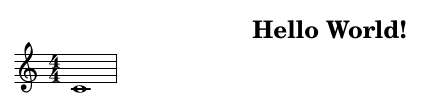
\includegraphics{HelloWorld.png}

\begin{lstlisting}[language=MusicXML, caption={\tt HelloWorld.xml}]
<?xml version="1.0" encoding="UTF-8" standalone="no"?>
<!DOCTYPE score-partwise PUBLIC
    "-//Recordare//DTD MusicXML 3.0 Partwise//EN"
    "http://www.musicxml.org/dtds/partwise.dtd">
<score-partwise version="3.0">
  <work>
    <work-title>Hello World!</work-title>
    </work>
  <!-- A very minimal MusicXML example -->
  <part-list>
    <score-part id="P1">
      <part-name>Music</part-name>
    </score-part>
  </part-list>
  <part id="P1">
<!--=========================================================-->
    <measure number="1">
  <!-- A very minimal MusicXML example, part P1, measure 1 -->
      <attributes>
        <divisions>1</divisions>
        <key>
          <fifths>0</fifths>
        </key>
        <time>
          <beats>4</beats>
          <beat-type>4</beat-type>
        </time>
        <clef>
          <sign>G</sign>
          <line>2</line>
        </clef>
      </attributes>
  <!-- A very minimal MusicXML example, part P1, measure 1, before first note -->
      <note>
        <pitch>
          <step>C</step>
          <octave>4</octave>
        </pitch>
        <duration>4</duration>
        <type>whole</type>
      </note>
    </measure>
<!--=========================================================-->
  </part>
</score-partwise>
\end{lstlisting}
%\end{figure}

\page


% -------------------------------------------------------------------------
% -------------------------------------------------------------------------
\section{Measurements}
% -------------------------------------------------------------------------
% -------------------------------------------------------------------------

% -------------------------------------------------------------------------
\subsection{Geometrical lengths}
% -------------------------------------------------------------------------

\mxml\ represents lengths by 10$^{th}$ of an interline space, i.e. the distance between lines in staves. This relative measure unit has the advantage that it allows all lengths to be represented independantly of the actual size of the score.

\sep

In \gitschemafile{common.mod} we find:

\begin{lstlisting}[language=MusicXML,caption={Relative lengths}]
<!--
	The tenths entity is a number representing tenths of
	interline space (positive or negative) for use in
	attributes. The layout-tenths entity is the same for
	use in elements. Both integer and decimal values are
	allowed, such as 5 for a half space and 2.5 for a
	quarter space. Interline space is measured from the
	middle of a staff line.
-->
<!ENTITY % tenths "CDATA">
<!ENTITY % layout-tenths "(#PCDATA)">
\end{lstlisting}

\sep

In order to obtain absolute lengths for \drawing, \mxml\ specifies how many tenths are equal to how many millimeters in the '{\tt <scaling>}' element, defined in \gitschemafile{layout.mod}:

\begin{lstlisting}[language=MusicXML,caption={Abolute lengths}]
<!--
	Version 1.1 of the MusicXML format added layout information
	for pages, systems, staffs, and measures. These layout
	elements joined the print and sound elements in providing
	formatting data as elements rather than attributes.

	Everything is measured in tenths of staff space. Tenths are
	then scaled to millimeters within the scaling element, used
	in the defaults element at the start of a score. Individual
	staves can apply a scaling factor to adjust staff size.
	When a MusicXML element or attribute refers to tenths,
	it means the global tenths defined by the scaling element,
	not the local tenths as adjusted by the staff-size element.
-->

<!-- .................. -->

<!--
	Margins, page sizes, and distances are all measured in
	tenths to keep MusicXML data in a consistent coordinate
	system as much as possible. The translation to absolute
	units is done in the scaling element, which specifies
	how many millimeters are equal to how many tenths. For
	a staff height of 7 mm, millimeters would be set to 7
	while tenths is set to 40. The ability to set a formula
	rather than a single scaling factor helps avoid roundoff
	errors.
-->
<!ELEMENT scaling (millimeters, tenths)>
<!ELEMENT millimeters (\#PCDATA)>
<!ELEMENT tenths %layout-tenths;>
\end{lstlisting}

\page

This leads for example to:
\begin{lstlisting}[language=MusicXML, caption={Scaling example}]
        <scaling>
          <millimeters>7.05556</millimeters>
          <tenths>40</tenths>
        </scaling>
\end{lstlisting}


% -------------------------------------------------------------------------
\subsection{Notes durations}
% -------------------------------------------------------------------------

\mxml\ uses a quantization of the duration with the '{\tt <divisions>}' element, which tells how many divisions there are in a quarter note:
\begin{lstlisting}[language=MusicXML]
       <divisions>2</divisions>
\end{lstlisting}

\sep

This example means that there are '{\tt 2}' divisions in a quarter note, i.e. the duration measure unit is an eigth note. Let's borrow from physics and MIDI terminology and call this a \MainIt{quantum}.

Any multiple of this quantum can be used in the \mxml\ data after that specification, but there's no way to express a duration less than an eigth node.

The quantum value has to be computed from the shortest note in the music that follows this element, taking tuplets into account, see section \mylink{tuplets}.

\sep

Is it possible to set the quantum to other values in multiple places in the \mxml\ data at will if needed? The DTD doesn't mentions that, and in practice, all applications support this feature.

\sep

Notes prolongation dots are specified with as many '{\tt <dot>}' elements as needed:
\begin{lstlisting}[language=MusicXML]
<!--
	One dot element is used for each dot of prolongation.
	The placement element is used to specify whether the
	dot should appear above or below the staff line. It is
	ignored for notes that appear on a staff space.
-->
<!ELEMENT dot EMPTY>
<!ATTLIST dot
    %print-style;
    %placement;
>
\end{lstlisting}


% -------------------------------------------------------------------------
\subsection{Graphics and sound}
% -------------------------------------------------------------------------

\mxml\ has to account for the possible difference between the drawn head note and the duration of that note, as is the case in tuplets.

In a tuplet containing 3 sixteenth notes, the duration of each such note is one third of that of an eigth note, but the drawn head note's graphical duration is half of that of the latter.
See section \mylink{tuplets}, for an example of how this is represented.

Some elements in \mxml\ data are specifically meant for MIDI support: they refer to the sound durations only.


% -------------------------------------------------------------------------
% -------------------------------------------------------------------------
\section{Measures}
\mylabel{mesures}
% -------------------------------------------------------------------------
% -------------------------------------------------------------------------

The '{\tt <measure>}' elements can contain many other elements, depending on the music.

Full measures are usually numbered from '{\tt 1}' up, but these numbers are actually character strings, \MainIt{not integers}: this allows for special measure numbers such as '{\tt X1}', for example, in the case of cue staves.

\sep

Anacruses are best specified "the purist way", with '{\tt 0}' as their number and the '{\tt implicit}' attribute set to '{\tt yes}', which specifies that this measure number should not be printed. One sees cases where the number is '{\tt 1}' for anacruses, though:
\begin{lstlisting}[language=MusicXML]
    <measure number="0" implicit="yes" width="129.48">
\end{lstlisting}

\sep

Measures can be irregular, i.e. with less total duration as the current time signature, or much longer that the usual time signatures, see \mylink{lyrics}, for an example.


% -------------------------------------------------------------------------
% -------------------------------------------------------------------------
\section{Elements attachment decisions}
% -------------------------------------------------------------------------
% -------------------------------------------------------------------------

The \mxml\ designers had to decide what element a given element should be attached to. Should a '{\tt <dynamics>}' element or '{\tt <metronome>}' element be attached to a note or be placed at the '{\tt <measure>}' level? Is so, should it occur in the data before or after the note over or below which it should be displayed?

\sep

\mxml\ defines a \MainIt{direction} as a musical indication that is not necessarily
	attached to a specific note. Two or more directions may be combined to
	indicate the start and stop of wedges, dashes, and so on.

\sep

For example, '{\tt <dynamics>}' elements are placed outside of '{\tt <note>}' elements in a '{\tt <direction>}' element, at the measure level:
\begin{lstlisting}[language=MusicXML]
      <direction placement="below">
        <direction-type>
          <dynamics>
            <ffff/>
          </dynamics>
        </direction-type>
        <staff>1</staff>
      </direction>
\end{lstlisting}

\sep

The elements attached to notes are placed inside a '{\tt <notations>}' element, itself placed inside a '{\tt <note>}' element. Notations are defined in \gitschemafile{note.mod}:
\begin{lstlisting}[language=MusicXML, caption={Notations definition}]
<!--
	Notations are musical notations, not XML notations. Multiple
	notations are allowed in order to represent multiple editorial
	levels. The print-object attribute, added in Version 3.0,
	allows notations to represent details of performance technique,
	such as fingerings, without having them appear in the score.
-->
<!ELEMENT notations
	(%editorial;,
	 (tied | slur | tuplet | glissando | slide |
	  ornaments | technical | articulations | dynamics |
	  fermata | arpeggiate | non-arpeggiate |
	  accidental-mark | other-notation)*)>
<!ATTLIST notations
    %print-object;
    %optional-unique-id;
>
\end{lstlisting}

\page


% -------------------------------------------------------------------------
% -------------------------------------------------------------------------
\section{Score description structure}
% -------------------------------------------------------------------------
% -------------------------------------------------------------------------

\mxml\ data contains a mix of legal informations, score geometry and musical contents. Some aspects of this are presented in this section.


% -------------------------------------------------------------------------
\subsection{Identification, rights and credits}
% -------------------------------------------------------------------------

The '{\tt  <identification>}' element is defined in \gitschemafile{identity.mod}:
\begin{lstlisting}[language=MusicXML]
<!--
	Identification contains basic metadata about the score.
	It includes the information in MuseData headers that
	may apply at a score-wide, movement-wide, or part-wide
	level. The creator, rights, source, and relation elements
	are based on Dublin Core.
-->
<!ELEMENT identification (creator*, rights*, encoding?,
	source?, relation*, miscellaneous?)>
\end{lstlisting}

\sep

For example, \gitmxmlfile{xmlsamples3.1/ActorPreludeSample.xml} contains:
\begin{lstlisting}[language=MusicXML,caption={Identification and rights example}]
  <identification>
    <creator type="composer">Lee Actor</creator>
    <rights>© 2004 Polygames.     All Rights Reserved.</rights>
    <encoding>
      <software>Finale v25 for Mac</software>
      <encoding-date>2017-12-12</encoding-date>
      <supports attribute="new-system" element="print" type="yes" value="yes"/>
      <supports attribute="new-page" element="print" type="yes" value="yes"/>
      <supports element="accidental" type="yes"/>
      <supports element="beam" type="yes"/>
      <supports element="stem" type="yes"/>
    </encoding>
  </identification>
\end{lstlisting}

\sep

The '{\tt <credit>}' element, defined in \gitschemafile{score.mod}, represents various legal informations about the score. It contains placement indication such as page number and alignment, as well as fonts information.

\sep

For example, one finds in \gitmxmlfile{xmlsamples3.1/ActorPreludeSample.xml}:
\begin{lstlisting}[language=MusicXML,caption={Credits example}]
  <credit page="1">
    <credit-type>title</credit-type>
    <credit-words default-x="1447" default-y="3477" font-size="19.5" justify="center" valign="top">Prelude to a Tragedy</credit-words>
  </credit>
  <credit page="1">
    <credit-type>composer</credit-type>
    <credit-words default-x="2718" default-y="3387" font-size="7.8" justify="right" valign="top">Lee Actor (2003)</credit-words>
  </credit>
  <credit page="1">
    <credit-type>rights</credit-type>
    <credit-words default-x="1447" default-y="45" font-size="7.8" justify="center" valign="bottom" xml:space="preserve">© 2004 Polygames.     All Rights Reserved.</credit-words>
  </credit>
  <credit page="2">
    <credit-type>page number</credit-type>
    <credit-words default-x="1412" default-y="45" font-size="7.8" halign="center" valign="bottom">- 2 -</credit-words>
  </credit>
  <credit page="3">
    <credit-type>page number</credit-type>
    <credit-words default-x="1447" default-y="45" font-size="7.8" halign="center" valign="bottom">- 3 -</credit-words>
  </credit>
  <credit page="4">
    <credit-type>page number</credit-type>
    <credit-words default-x="1412" default-y="45" font-size="7.8" halign="center" valign="bottom">- 4 -</credit-words>
  </credit>
\end{lstlisting}

\sep

We see the '{\tt <credit-words>}' element in the example above. In \mxml, '{\tt words}' means text, as defined in \gitschemafile{direction.mod}:
\begin{lstlisting}[language=MusicXML]
<!--
	The words element specifies a standard text direction.
	Left justification is assumed if not specified.
	Language is Italian ("it") by default. Enclosure
	is none by default.
-->
<!ELEMENT words (#PCDATA)>
<!ATTLIST words
    %text-formatting;
    %optional-unique-id;
>
\end{lstlisting}


% -------------------------------------------------------------------------
\subsection{Score geometry}
% -------------------------------------------------------------------------

The dimensions and margins of the graphics score can be specified with the '{\tt <page-layout>}' element, as in \gitmxmlfile{basic/ClefKeyTime.xml}:
\begin{lstlisting}[language=MusicXML, caption={Page layout example}]
  <defaults>
    <scaling>
      <millimeters>7.05556</millimeters>
      <tenths>40</tenths>
      </scaling>
    <page-layout>
      <page-height>1683.36</page-height>
      <page-width>1190.88</page-width>
      <page-margins type="even">
        <left-margin>56.6929</left-margin>
        <right-margin>56.6929</right-margin>
        <top-margin>56.6929</top-margin>
        <bottom-margin>113.386</bottom-margin>
        </page-margins>
      <page-margins type="odd">
        <left-margin>56.6929</left-margin>
        <right-margin>56.6929</right-margin>
        <top-margin>56.6929</top-margin>
        <bottom-margin>113.386</bottom-margin>
        </page-margins>
      </page-layout>
    <word-font font-family="FreeSerif" font-size="10"/>
    <lyric-font font-family="FreeSerif" font-size="11"/>
    </defaults>
\end{lstlisting}


% -------------------------------------------------------------------------
\subsection{Part groups and parts}
% -------------------------------------------------------------------------

Part groups are used to structure complex scores, mimicking the way large orchestras are organized. For example, there can be a winds group, containing several groups such as flutes, oboes, horns and bassoons.

\sep

A '{\tt <part-group>}' element has a '{\tt type}' attribute, whose value can be '{\tt start}' or '{\tt stop}'. A~part group is thus delimited by a pair of '{\tt <part-group>}' elements, the first one of type '{\tt start}', and the second one of type '{\tt stop}'.

The '{\tt id}' attribute of the '{\tt <score-part>}' element is used to reference the part later in the \mxml\ data. Often, is has the form '{\tt Pn}', where '{\tt n}' is a number.

\sep

Part groups can be nested, leading to a hierarchy of groups. This is done with the '{\tt number}' attribute of the '{\tt <part-group>}' element, which indicates how '{\tt start}' and '{\tt stop}' attributes are paired together.

\sep

For example, \gitmxmlfile{partgroups/NestedPartGroups.xml} contains:\\
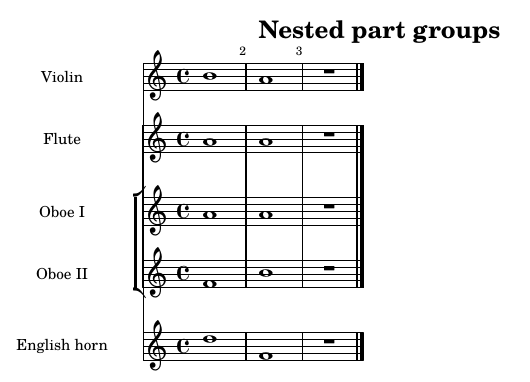
\includegraphics[scale=0.7]{NestedPartGroups.png}

\begin{lstlisting}[language=MusicXML, caption={Nested part groups example}]
  <part-list>
    <score-part id="P1">
      <part-name>Violin</part-name>
    </score-part>
    <part-group number="1" type="start">
      <group-symbol>line</group-symbol>
      <group-barLine>yes</group-barLine>
    </part-group>
    <score-part id="P2">
      <part-name>Flute</part-name>
    </score-part>
    <part-group number="2" type="start">
      <group-symbol>bracket</group-symbol>
      <group-barLine>yes</group-barLine>
    </part-group>
    <score-part id="P3">
      <part-name>Oboe I</part-name>
    </score-part>
    <score-part id="P4">
      <part-name>Oboe II</part-name>
    </score-part>
    <part-group number="2" type="stop"/>
    <part-group number="1" type="stop"/>
    <score-part id="P5">
      <part-name>English horn</part-name>
    </score-part>
  </part-list>
\end{lstlisting}

\sep

The \mxml\ DTD states that part groups may \MainIt{overlap}. This author suspects that this is only because Finale\texttrademark\ doesn't create \mxml\ markups in a strict first-in, last-out order.

\sep

Various applications handle \gitmxmlfile{lilypond-ignored/OverlappingPartGroups.xml} their own way. \xmlToLy\ rejects such data for the time being, with this message:
\begin{lstlisting}[language=MusicXML,caption={Overlapping groups \xmlToLy\ error message}]
  ### MusicXML ERROR ### lilypond-ignored/OverlappingPartGroups.xml:39:
There are overlapping part groups, namely:
  '1' -=> PartGroup_2 ('1', partGroupName "Part group 1"), lines 15..39
and
  '2' -=> PartGroup_3 ('2', partGroupName "Part group 2"), lines 27..43

Please contact the maintainers of MusicFormats (see option '-c, -contact'):
  either you found a bug in the xml2ly converter,
  or this MusicXML data is the first-ever real-world case
  of a score exhibiting overlapping part groups
Abort trap: 6 (core dumped)
\end{lstlisting}


% -------------------------------------------------------------------------
\subsection{Staves and voices}
% -------------------------------------------------------------------------

In \mxml, a part is composed of one or more staves, each composed of one or more voices.
There are no structured staves nor voices as such in \mxml\ however -- that is, not the way parts and measures are. The '{\tt <stave>}' and '{\tt voice}' element only contain a number.

\sep

To be more precise:
\begin{itemize}
\item stave numbers start at '{\tt 1}' in every part, which refers to the top-most staff in the part;

\item a staff number of '{\tt 1}' is implied by default, i.e. when an optional '{\tt <stave>}' element is missing, as can happen in notes descriptions;

\item voice numbers start at '{\tt 1}' in every staff, and a voice number of '{\tt 1}' is implied by default, i.e. when an optional '{\tt <voice>}' element is missing;
\end{itemize}

A given voice can change staff and come back to the former one, for example in keyboard scores.

\sep

This author has found \mxml\ files in which the voice numbers are not contiguous, such as '{\tt 1}', '{\tt 5}' and '{\tt 9}'. The DTD doesn't preclude this, and the applications handle example \gitmxmlfile{multistaff/NonContiguousVoiceNumbers.xml} their own way.


% -------------------------------------------------------------------------
\subsection{Clefs, keys and time signatures}
% -------------------------------------------------------------------------

\mxml\ offers elements to describe the common cases:
\begin{itemize}
\item traditional keys are described by a '{\tt <fifths>}' element;

\item simple clefs are described by '{\tt <sign>}' and '{\tt <line>}' elements;

\item simple time signatures are desribed by '{\tt <beats>}' and '{\tt <beat-type>}' elements.
\end{itemize}

\page

An example is found in \gitmxmlfile{basic/ClefKeyTime.xml}:\\
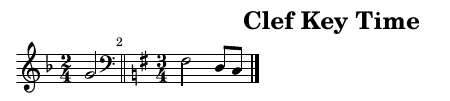
\includegraphics{ClefKeyTime.png}
\begin{lstlisting}[language=MusicXML, caption={Clef, key and time signature example}]
      <attributes>
        <divisions>2</divisions>
        <key>
          <fifths>-1</fifths>
          </key>
        <time>
          <beats>2</beats>
          <beat-type>4</beat-type>
          </time>
        <clef>
          <sign>G</sign>
          <line>2</line>
          </clef>
        </attributes>
      <!-- ... ... ... ... ... -->
      <attributes>
        <key>
          <fifths>1</fifths>
          </key>
        <time>
          <beats>3</beats>
          <beat-type>4</beat-type>
          </time>
        <clef>
          <sign>F</sign>
          <line>4</line>
          </clef>
        </attributes>
\end{lstlisting}

\sep

In this example, the various sub-elements are:
%\begin{adjustwidth}{-0.5cm}{-0.5cm}
\begin{center}
\footnotesize
\def \contentsWidth{0.5\textwidth}
\def \arraystretch{1.3}
%
\begin{tabular}[t]{lp{\contentsWidth}}
\textbf{Fragment}&\textbf{Meaning} \tabularnewline[0.5ex]
\hline\\[-3.0ex]
%
'{\tt  <fifths>-1</fifths>}' & the number of fitfhs. A negative number is the number of flats, 0 means C major or A minor, and a positive value is the number of sharps
\tabularnewline

'{\tt <beats>2</beats>}' & the number of beats per measure \tabularnewline

'{\tt <beat-type>4</beat-type>}' & the beat type, i.e. the duration of each beat expressed as a fraction of a whole note
\tabularnewline

'{\tt <sign>G</sign>}' & the clef sign to be displayed. Sign values include '{\tt G}', '{\tt F}', '{\tt C}',
	'{\tt percussion}', '{\tt TAB}', '{\tt jianpu}', and '{\tt none}'
\tabularnewline

'{\tt <line>2</line>}' & the number of the line at which the clef is placed
\tabularnewline

\end{tabular}
\end{center}
%\end{adjustwidth}

\sep

Composite time signatures such as '{\tt 2/4 + 3/8}' and '{\tt 3+2/8}' can be specified, as well as '{\tt <senza-misura>}' for cadenzas.

\page

\mxml\ also supports non-traditional keys the Humdrum/Scot way. For example, the time signature at the beginning of measure 2 in \gitmxmlfile{keys/HumdrumScotKeys.xml} is described by:\\
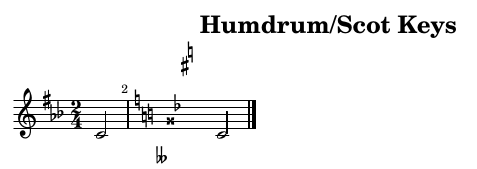
\includegraphics{HumdrumScotKeys.png}

\begin{lstlisting}[language=MusicXML, caption={Humdrum/Scot non-traditional key example}]
        <key>
          <key-step>C</key-step>
          <key-alter>-2</key-alter>
          <key-step>G</key-step>
          <key-alter>2</key-alter>
          <key-step>D</key-step>
          <key-alter>-1</key-alter>
          <key-step>B</key-step>
          <key-alter>1</key-alter>
          <key-step>F</key-step>
          <key-alter>0</key-alter>
          <key-octave number="1">2</key-octave>
          <key-octave number="2">3</key-octave>
          <key-octave number="3">4</key-octave>
          <key-octave number="4">5</key-octave>
          <key-octave number="5">6</key-octave>
        </key>
\end{lstlisting}

This is another example handled diffently by some applications.


% -------------------------------------------------------------------------
\subsection{Metromone and tempo}
% -------------------------------------------------------------------------

\mxml\ has rich support for metronome specifications. Example \gitmxmlfile{tempos/SwingTempo.xml} contains:\\
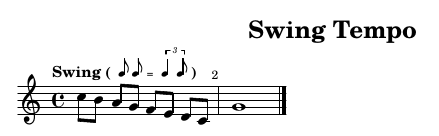
\includegraphics{SwingTempo.png}.
\begin{lstlisting}[language=MusicXML,caption={Swing tempo example}]
     <direction placement="above">
        <direction-type>
          <words>Swing</words>
        </direction-type>
        <direction-type>
          <metronome parentheses="yes" default-y="30" halign="left" relative-x="26">
            <metronome-note>
              <metronome-type>eighth</metronome-type>
              <metronome-beam number="1">begin</metronome-beam>
            </metronome-note>
            <metronome-note>
              <metronome-type>eighth</metronome-type>
              <metronome-beam number="1">end</metronome-beam>
            </metronome-note>
            <metronome-relation>equals</metronome-relation>
            <metronome-note>
              <metronome-type>quarter</metronome-type>
              <metronome-tuplet bracket="yes" show-number="actual" type="start">
                <actual-notes>3</actual-notes>
                <normal-notes>2</normal-notes>
                <normal-type>eighth</normal-type>
              </metronome-tuplet>
            </metronome-note>
            <metronome-note>
              <metronome-type>eighth</metronome-type>
              <metronome-tuplet type="stop">
                <actual-notes>3</actual-notes>
                <normal-notes>2</normal-notes>
                <normal-type>eighth</normal-type>
              </metronome-tuplet>
            </metronome-note>
          </metronome>
        </direction-type>
      </direction>
\end{lstlisting}


% -------------------------------------------------------------------------
% -------------------------------------------------------------------------
\section{Notes}
% -------------------------------------------------------------------------
% -------------------------------------------------------------------------

A note is described by a '{\tt note}' element, defined in \gitschemafile{note.mod}:
\begin{lstlisting}[language=MusicXML, caption={Note definition}]
<!--
	Notes are the most common type of MusicXML data. The
	MusicXML format keeps the MuseData distinction between
	elements used for sound information and elements used for
	notation information (e.g., tie is used for sound, tied for
	notation). Thus grace notes do not have a duration element.
	Cue notes have a duration element, as do forward elements,
	but no tie elements. Having these two types of information
	available can make interchange considerably easier, as
	some programs handle one type of information much more
	readily than the other.
-->
<!ELEMENT note
	(((grace, ((%full-note;, (tie, tie?)?) | (cue, %full-note;))) |
	  (cue, %full-note;, duration) |
	  (%full-note;, duration, (tie, tie?)?)),
	 instrument?, %editorial-voice;, type?, dot*,
	 accidental?, time-modification?, stem?, notehead?,
	 notehead-text?, staff?, beam*, notations*, lyric*, play?)>
\end{lstlisting}


\sep

Consider \gitmxmlfile{basic/MinimalScore.xml}:\\
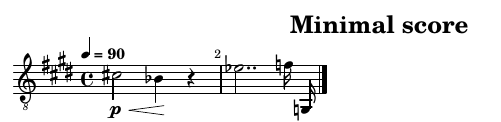
\includegraphics{MinimalScore.png}

\page

The first note in measure 2 in this example is described by:
\begin{lstlisting}[language=MusicXML, caption={Minimal score example}]
        <divisions>8</divisions>

      <!-- ... ... ... ... ... -->

        <clef>
          <sign>G</sign>
          <line>2</line>
          <clef-octave-change>-1</clef-octave-change>
        </clef>

      <!-- ... ... ... ... ... -->

      <note>
        <pitch>
          <step>E</step>
          <alter>-1</alter>
          <octave>4</octave>
        </pitch>
        <duration>28</duration>
        <voice>1</voice>
        <type>half</type>
        <dot />
        <dot />
        <accidental>flat</accidental>
      </note>
\end{lstlisting}

\sep

In this example, the various sub-elements are:
%\begin{adjustwidth}{-0.5cm}{-0.5cm}
\begin{center}
\footnotesize
\def \contentsWidth{0.5\textwidth}
\def \arraystretch{1.3}
%
\begin{tabular}[t]{lp{\contentsWidth}}
\textbf{Fragment}&\textbf{Meaning} \tabularnewline[0.5ex]
\hline\\[-3.0ex]
%
'{\tt <step>E</step>}' & the diatonic pitch of the note, from A to G
\tabularnewline

'{\tt <alter>-1</alter>}' & the chromatic alteration in
	number of semitones (e.g., -1 for flat, 1 for sharp)
\tabularnewline

'{\tt <octave>4</octave>}' & the absolute octave of the note, 0 to 9, where 4 indicates the octave
	started by middle C
\tabularnewline

'{\tt <duration>28</duration>}' & the sounding duration of the note, 28 quanta, which is a double dotted half note with 4 quanta per quarter note (16+8+4)
\tabularnewline

'{\tt <voice>1</voice>}' & the voice number of the note, 1
\tabularnewline

'{\tt <type>half</type>}' & the display duration of the note, a half note, which determines the note head
\tabularnewline

\end{tabular}
\end{center}
%\end{adjustwidth}

Middle C is the one between the left hand and right hand staves in a typical score. Note here: octave numbers are absolute, and the treble clef is octaviated by a '{\tt <clef-octave-change>}' element!

Voice and staff numbers are optional, in which case the default value is 1.

\sep

Having both a sounding and display duration specification is necessary because they do not coincide in the case of dotted notes and tuplets members, see \mylink{tuplets}, for the latter.

\page

Note elements can have '{\tt <stem>}' and '{\tt <beam>}' sub-elements attached to them, as in the following example. See \mylink{graceNotes} for a score containing some:
\begin{lstlisting}[language=MusicXML]
      <note>
        <pitch>
          <step>A</step>
          <octave>2</octave>
        </pitch>
        <voice>3</voice>
        <type>16th</type>
        <stem>up</stem>
        <staff>2</staff>
        <beam number="1">begin</beam>
        <beam number="2">begin</beam>
      </note>
\end{lstlisting}

\sep

Before showing an example, we shall look into more detail in the elements that are attached to notes in the forthcoming sections.


% -------------------------------------------------------------------------
\subsection{Accidentals}
% -------------------------------------------------------------------------

\begin{lstlisting}[language=MusicXML]
<!--
	Actual notated accidentals. Valid values include: sharp,
	natural, flat, double-sharp, sharp-sharp, flat-flat,
	natural-sharp, natural-flat, quarter-flat, quarter-sharp,
	three-quarters-flat, three-quarters-sharp, sharp-down,
	sharp-up, natural-down, natural-up, flat-down, flat-up,
	double-sharp-down, double-sharp-up, flat-flat-down,
	flat-flat-up, arrow-down, arrow-up, triple-sharp,
	triple-flat, slash-quarter-sharp, slash-sharp, slash-flat,
	double-slash-flat, sharp-1, sharp-2, sharp-3, sharp-5,
	flat-1, flat-2, flat-3, flat-4, sori, koron, and other.
	... ... ... ... ...
-->
<!ELEMENT accidental (#PCDATA)>
<!ATTLIST accidental
    cautionary %yes-no; #IMPLIED
    editorial %yes-no; #IMPLIED
    %level-display;
    %print-style;
    %smufl;
>
\end{lstlisting}


% -------------------------------------------------------------------------
\subsection{Articulations}
% -------------------------------------------------------------------------
The \mxml\ articulation elementss are:
\begin{lstlisting}[language=MusicXML]
<!--
	Articulations and accents are grouped together here.
-->
<!ELEMENT articulations
	((accent | strong-accent | staccato | tenuto |
	  detached-legato | staccatissimo | spiccato |
	  scoop | plop | doit | falloff | breath-mark |
	  caesura | stress | unstress | soft-accent |
	  other-articulation)*)>
<!ATTLIST articulations
    %optional-unique-id;
>
\end{lstlisting}


% -------------------------------------------------------------------------
\subsection{Ornaments}
% -------------------------------------------------------------------------

Ornaments are defined in \gitschemafile{note.mod}:
\begin{lstlisting}[language=MusicXML]
<!ELEMENT ornaments
	(((trill-mark | turn | delayed-turn | inverted-turn |
	   delayed-inverted-turn | vertical-turn |
	   inverted-vertical-turn | shake | wavy-line |
	   mordent | inverted-mordent | schleifer | tremolo |
	   haydn | other-ornament), accidental-mark*)*)>
<!ATTLIST ornaments
    %optional-unique-id;
>
<!ELEMENT trill-mark EMPTY>
<!ATTLIST trill-mark
    %print-style;
    %placement;
    %trill-sound;
>
\end{lstlisting}


% -------------------------------------------------------------------------
\subsection{Dynamics}
% -------------------------------------------------------------------------

\mxml\ dynamics are defined in \gitschemafile{common.mod}:

\begin{lstlisting}[language=MusicXML]
<!ELEMENT dynamics ((p | pp | ppp | pppp | ppppp | pppppp |
	f | ff | fff | ffff | fffff | ffffff | mp | mf | sf |
	sfp | sfpp | fp | rf | rfz | sfz | sffz | fz |
	n | pf | sfzp | other-dynamics)*)>
<!ATTLIST dynamics
    %print-style-align;
    %placement;
    %text-decoration;
    %enclosure;
    %optional-unique-id;
\end{lstlisting}

Other dynamics can also be specified:
\begin{lstlisting}[language=MusicXML]
The other-dynamics element
	allows other dynamic marks that are not covered here, but
	many of those should perhaps be included in a more general
	musical direction element. Dynamics may also be combined as
	in <sf/><mp/>.
\end{lstlisting}


% -------------------------------------------------------------------------
\subsection{An example of articulations and dynamics}
% -------------------------------------------------------------------------

The reader can see various such in \gitmxmlfile{articulations/ArticulationsAndOrnaments.xml}:\\
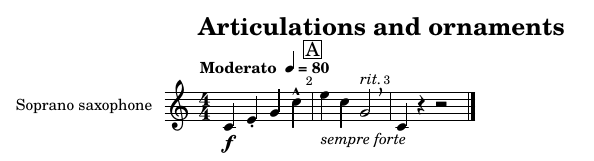
\includegraphics{ArticulationsAndOrnaments.png}

\page


% -------------------------------------------------------------------------
\subsection{Grace notes}
\mylabel{graceNotes}
% -------------------------------------------------------------------------

The '{\tt <grace>}' element is defined in \gitschemafile{note.mod}:
\begin{lstlisting}[language=MusicXML]
<!--
	The grace element indicates the presence of a grace note.
	The slash attribute for a grace note is yes for slashed
	eighth notes. The other grace note attributes come from
	MuseData sound suggestions. The steal-time-previous attribute
	indicates the percentage of time to steal from the previous
	note for the grace note. The steal-time-following attribute
	indicates the percentage of time to steal from the following
	note for the grace note, as for appoggiaturas. The make-time
	attribute indicates to make time, not steal time; the units
	are in real-time divisions for the grace note.
-->
<!ELEMENT grace EMPTY>
<!ATTLIST grace
    steal-time-previous CDATA #IMPLIED
    steal-time-following CDATA #IMPLIED
    make-time CDATA #IMPLIED
    slash %yes-no; #IMPLIED
>
\end{lstlisting}

\sep

For example, in \gitmxmlfile{gracenotes/LilyPondIssue34.xml}, the three grace notes at the beginning of the lower staff are described by:\\
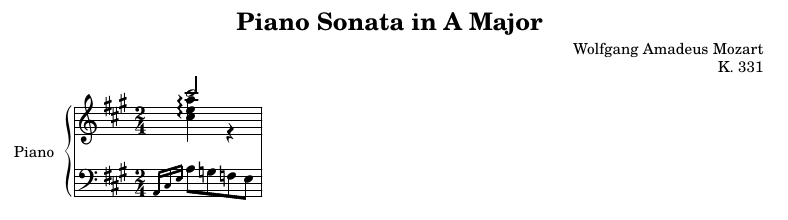
\includegraphics[scale=0.85]{LilyPondIssue34.png}
\begin{lstlisting}[language=MusicXML,caption={Grace notes example}]
      <note>
        <grace/>
        <pitch>
          <step>A</step>
          <octave>2</octave>
        </pitch>
        <voice>3</voice>
        <type>16th</type>
        <stem>up</stem>
        <staff>2</staff>
        <beam number="1">begin</beam>
        <beam number="2">begin</beam>
        <notations>
          <slur type="start" placement="above" number="1"/>
        </notations>
      </note>
      <note>
        <grace/>
        <pitch>
          <step>C</step>
          <alter>1</alter>
          <octave>3</octave>
        </pitch>
        <voice>3</voice>
        <type>16th</type>
        <stem>up</stem>
        <staff>2</staff>
        <beam number="1">continue</beam>
        <beam number="2">continue</beam>
      </note>
      <note>
        <grace/>
        <pitch>
          <step>E</step>
          <octave>3</octave>
        </pitch>
        <voice>3</voice>
        <type>16th</type>
        <stem>up</stem>
        <staff>2</staff>
        <beam number="1">end</beam>
        <beam number="2">end</beam>
      </note>
\end{lstlisting}


% -------------------------------------------------------------------------
% -------------------------------------------------------------------------
\section{Ties}
% -------------------------------------------------------------------------
% -------------------------------------------------------------------------

\mxml\ makes the distinction between graphics and sound, and this applied to ties: the '{\tt <tie>}' element indicates sound, and the '{\tt <tied>}'	element indicates notation. In a '{\tt <tie>}', the '{\tt start}' and '{\tt stop}' values in the '{\tt type}' attribute are used to indicate the beginning and end of the tie.

\sep

These two elements are defined in \gitschemafile{note.mod}:
\begin{lstlisting}[language=MusicXML]
<!ELEMENT tie EMPTY>
<!ATTLIST tie
    type %start-stop; #REQUIRED
    %time-only;
\end{lstlisting}

\begin{lstlisting}[language=MusicXML]
<!ELEMENT tied EMPTY>
<!ATTLIST tied
    type %tied-type; #REQUIRED
    number %number-level; #IMPLIED
    %line-type;
    %dashed-formatting;
    %position;
    %placement;
    %orientation;
    %bezier;
    %color;
    %optional-unique-id;
>
\end{lstlisting}


% -------------------------------------------------------------------------
% -------------------------------------------------------------------------
\section{Slurs}
% -------------------------------------------------------------------------
% -------------------------------------------------------------------------

The '{\tt <slur>}' element is placed inside a '{\tt <notations>}' element, itself placed inside a '{\tt <note>}' element.  It is defined in \gitschemafile{note.mod}:
\begin{lstlisting}[language=MusicXML]
<!ELEMENT slur EMPTY>
<!ATTLIST slur
    type %start-stop-continue; #REQUIRED
    number %number-level; "1"
    %line-type;
    %dashed-formatting;
    %position;
    %placement;
    %orientation;
    %bezier;
    %color;
    %optional-unique-id;
>
\end{lstlisting}


% -------------------------------------------------------------------------
% -------------------------------------------------------------------------
\section{Tie and slur example}
% -------------------------------------------------------------------------
% -------------------------------------------------------------------------

This example is in \gitmxmlfile{basic/TieAndSlur.xml}:\\
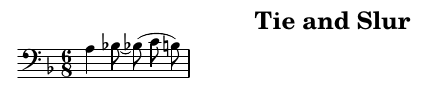
\includegraphics{TieAndSlur.png}

\sep

\begin{lstlisting}[language=MusicXML, caption={Tie and slur example}]
      <note>
        <pitch>
          <step>A</step>
          <octave>3</octave>
        </pitch>
        <duration>2</duration>
        <type>quarter</type>
        <voice>1</voice>
      </note>
      <note>
        <pitch>
          <step>B</step>
          <alter>-1</alter>
          <octave>3</octave>
        </pitch>
        <duration>1</duration>
        <type>eighth</type>
        <voice>1</voice>
        <accidental>flat</accidental>
        <tie type="start" />
        <notations>
          <tied type="start" />
        </notations>
      </note>
      <note>
        <pitch>
          <step>B</step>
          <alter>-1</alter>
          <octave>3</octave>
        </pitch>
        <duration>1</duration>
        <type>eighth</type>
        <voice>1</voice>
        <accidental>flat</accidental>
        <tie type="stop" />
        <notations>
          <tied type="stop" />
          <slur number="1" type="start" />
        </notations>
      </note>
      <note>
        <pitch>
          <step>C</step>
          <octave>4</octave>
        </pitch>
        <duration>1</duration>
        <type>eighth</type>
        <voice>1</voice>
      </note>
      <note>
        <pitch>
          <step>B</step>
          <octave>3</octave>
        </pitch>
        <duration>1</duration>
        <type>eighth</type>
        <voice>1</voice>
        <notations>
          <slur number="1" type="stop" />
        </notations>
      </note>
\end{lstlisting}


%% -------------------------------------------------------------------------
%% -------------------------------------------------------------------------
%\section{Harmonies and figured bass}
%% -------------------------------------------------------------------------
%% -------------------------------------------------------------------------
%
%% -------------------------------------------------------------------------
%\section{Harmonies}
%% -------------------------------------------------------------------------
%
%The '{\tt <harmony>}' element in \mxml\ goes beyond merely displaying harmonies, since it can describe harmonic analysis. i.e. harmonies functions.
%
%Here is how it is defined in \gitschemafile{direction.mod}:
%
\begin{lstlisting}[language=MusicXML]
%<!--
%	The harmony elements are based on Humdrum's **harm
%	encoding, extended to support chord symbols in popular
%	music as well as functional harmony analysis in classical
%	music.
%
%	If there are alternate harmonies possible, this can be
%	specified using multiple harmony elements differentiated
%	by type. Explicit harmonies have all note present in the
%	music; implied have some notes missing but implied;
%	alternate represents alternate analyses.
%
%	The harmony object may be used for analysis or for
%	chord symbols. The print-object attribute controls
%	whether or not anything is printed due to the harmony
%	element. The print-frame attribute controls printing
%	of a frame or fretboard diagram. The print-style entity
%	sets the default for the harmony, but individual elements
%	can override this with their own print-style values.
%
%	A harmony element can contain many stacked chords (e.g.
%	V of II). A sequence of harmony-chord entities is used
%	for this type of secondary function, where V of II would
%	be represented by a harmony-chord with a V function
%	followed by a harmony-chord with a II function.
%-->
%<!ENTITY % harmony-chord "((root | function), kind,
%	inversion?, bass?, degree*)">
%
%<!ELEMENT harmony ((%harmony-chord;)+, frame?,
%	offset?, %editorial;, staff?)>
%<!ATTLIST harmony
%    type (explicit | implied | alternate) #IMPLIED
%    %print-object;
%    print-frame  %yes-no; #IMPLIED
%    %print-style;
%    %placement;
%    %optional-unique-id;
%>
%\end{lstlisting}
%
%
%% -------------------------------------------------------------------------
%\section{Figured bass}
%% -------------------------------------------------------------------------
%
%The '{\tt <figured-bass>}' element is defined in \gitschemafile{node.mod} this way:
%
\begin{lstlisting}[language=MusicXML]
%<!--
%	Figured bass elements take their position from the first
%	regular note (not a grace note or chord note) that follows
%	in score order. The optional duration element is used to
%	indicate changes of figures under a note.
%
%	Figures are ordered from top to bottom. A figure-number is
%	a number. Values for prefix and suffix include plus and
%	the accidental values sharp, flat, natural, double-sharp,
%	flat-flat, and sharp-sharp. Suffixes include both symbols
%	that come after the figure number and those that overstrike
%	the figure number. The suffix values slash, back-slash, and
%	vertical are used for slashed numbers indicating chromatic
%	alteration. The orientation and display of the slash usually
%	depends on the figure number. The prefix and suffix elements
%	may contain additional values for symbols specific to
%	particular figured bass styles. The value of parentheses
%	is "no" if not present.
%-->
%<!ELEMENT figured-bass (figure+, duration?, %editorial;)>
%<!ATTLIST figured-bass
%    %print-style;
%    %printout;
%    parentheses %yes-no; #IMPLIED
%    %optional-unique-id;
%>
%<!ELEMENT figure
%	(prefix?, figure-number?, suffix?, extend?, %editorial;)>
%<!ELEMENT prefix (#PCDATA)>
%<!ATTLIST prefix
%    %print-style;
%>
%<!ELEMENT figure-number (#PCDATA)>
%<!ATTLIST figure-number
%    %print-style;
%>
%<!ELEMENT suffix (#PCDATA)>
%<!ATTLIST suffix
%    %print-style;
%>
%\end{lstlisting}


% -------------------------------------------------------------------------
% -------------------------------------------------------------------------
\section{Chords}
% -------------------------------------------------------------------------
% -------------------------------------------------------------------------

Chords are not evidenced as such in \mxml\ data. Instead, the '{\tt <chord>}' element means that the given note is part of a chord after the first note in the chord has be met. Remember:~\mxml\ is about \drawing\ scores. Put it another way, you know there is a chord \MainIt{only upon its second note}.

\sep

The code for the last three note chord in \gitmxmlfile{chords/Chords.xml} is shown below.

%\begin{figure}
%\caption{Last chord from \gitmxmlfile{chords/Chords.xml}\mylabel{chords}
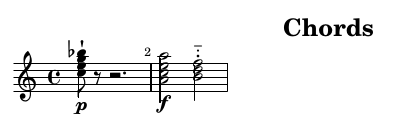
\includegraphics{Chords.png}

\begin{lstlisting}[language=MusicXML, caption={Chord example}]
      <note>
        <pitch>
          <step>B</step>
          <octave>4</octave>
        </pitch>
        <duration>4</duration>
        <voice>1</voice>
        <type>half</type>
        <notations>
          <articulations>
            <staccato />
            <detached-legato />
          </articulations>
        </notations>
      </note>
      <note>
        <chord />
        <pitch>
          <step>D</step>
          <octave>5</octave>
        </pitch>
        <duration>4</duration>
        <voice>1</voice>
        <type>half</type>
      </note>
      <note>
        <chord />
        <pitch>
          <step>F</step>
          <octave>5</octave>
        </pitch>
        <duration>4</duration>
        <voice>1</voice>
        <type>half</type>
      </note>
\end{lstlisting}
%\end{figure}


% -------------------------------------------------------------------------
% -------------------------------------------------------------------------
\section{Tuplets}
\mylabel{tuplets}
% -------------------------------------------------------------------------
% -------------------------------------------------------------------------

The situation for tuplets is different than that of the chords: there is a '{\tt <tuplet>}' element, with a '{\tt type}' attribute to indicate the note upon which it starts and stops:

\begin{lstlisting}[language=MusicXML]
        <notations>
          <tuplet number="1" type="start" />
        </notations>
\end{lstlisting}

The '{\tt number}' attribute can be used to describe nested tuplets:

The contents, i.e. the notes in the tuplet, are not nested in the latter: there are placed in sequence between the two '{\tt <tuplet>}' elements that delimitate the tuplet.

\sep

Each note in the tuplet has a '{\tt <time-modification>}' element, from the first one on. This element contains two elements:
\begin{lstlisting}[language=MusicXML]
        <time-modification>
          <actual-notes>3</actual-notes>
          <normal-notes>2</normal-notes>
        </time-modification>
\end{lstlisting}

One should play '{\tt <actual-notes>}' within the time taken by only '{\tt <normal-notes>}'. The example above is thus that of a triplet.

\sep

In the case of \gitmxmlfile{tuplets/Tuplets.xml}, shown below, the duration of the tuplets member is 20 quanta, i.e. 2/3 of a quarter note, whose duration is 30, and the 'display' duration is a quarter note. The duration of the triplet as a whole is that of a half note, i.e. 60 quanta.

%\begin{figure}
%\caption{First tuplet from \gitmxmlfile{tuplets/Tuplet.xml}}\mylabel{tuplets}
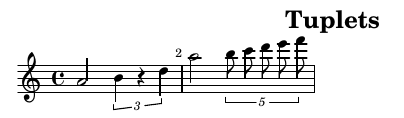
\includegraphics{Tuplets.png}

\begin{lstlisting}[language=MusicXML, caption={Tuplet example}]
        <divisions>30</divisions>

			<!-- ... ... ... ... ... -->

      <note>
        <pitch>
          <step>B</step>
          <octave>4</octave>
        </pitch>
        <duration>20</duration>
        <voice>1</voice>
        <type>quarter</type>
        <time-modification>
          <actual-notes>3</actual-notes>
          <normal-notes>2</normal-notes>
        </time-modification>
        <notations>
          <tuplet number="1" type="start" />
        </notations>
      </note>
      <note>
        <rest />
        <duration>20</duration>
        <voice>1</voice>
        <type>quarter</type>
        <time-modification>
          <actual-notes>3</actual-notes>
          <normal-notes>2</normal-notes>
        </time-modification>
      </note>
      <note>
        <pitch>
          <step>D</step>
          <octave>5</octave>
        </pitch>
        <duration>20</duration>
        <voice>1</voice>
        <type>quarter</type>
        <time-modification>
          <actual-notes>3</actual-notes>
          <normal-notes>2</normal-notes>
        </time-modification>
        <notations>
          <tuplet number="1" type="stop" />
        </notations>
      </note>
\end{lstlisting}
%\end{figure}


% -------------------------------------------------------------------------
% -------------------------------------------------------------------------
\section{BarLines and repeats}
% -------------------------------------------------------------------------
% -------------------------------------------------------------------------

Repeats are not described by high-level elements in \mxml. Instead, specific barLines containing a '{\tt <repeat>}' element are used to draw the necessary delimiters.


% -------------------------------------------------------------------------
\subsection{Simple barLines}
% -------------------------------------------------------------------------

The '{\tt <barLine>}' element is defined in \gitschemafile{barLine.mod}. It has two main attributes:
%\begin{adjustwidth}{-0.5cm}{-0.5cm}
\begin{center}
\footnotesize
\def \contentsWidth{0.5\textwidth}
\def \arraystretch{1.3}
%
\begin{tabular}[t]{lp{\contentsWidth}}
\textbf{Attribute}&\textbf{Meaning} \tabularnewline[0.5ex]
\hline\\[-3.0ex]
%
{\tt bar-style} & Bar-style contains style information. Choices are
	'{\tt regular}', '{\tt dotted}', '{\tt dashed}', '{\tt heavy}', '{\tt light-light}',
	'{\tt light-heavy}', '{\tt heavy-light}', '{\tt heavy-heavy}', '{\tt tick}' (a
	short stroke through the top line), '{\tt short}' (a partial
	barLine between the 2nd and 4th lines), and '{\tt none}'.

	BarLines can occur within measures, as in dotted
	barLines that subdivide measures in complex meters;
\tabularnewline

{\tt location} & If location is '{\tt left}',
	it should be the first element in the measure, aside from
	the '{\tt print}', '{\tt bookmark}', and '{\tt link}' elements.

	If location is
	'{\tt right}', it should be the last element, again with the
	possible std::exception of the '{\tt print}', '{\tt bookmark}', and '{\tt link}'
	elements.

	The value can be '{\tt right}', '{\tt left}' or '{\tt middle}'.
	If no location is specified, the default value is '{\tt right}'.
\tabularnewline

\end{tabular}
\end{center}
%\end{adjustwidth}

%The possible bar styles are defined in \gitschemafile{barLine.mod}:
%
\begin{lstlisting}[language=MusicXML,caption={Existing bar styles}]
%<!--
%	Bar-style contains style information. Choices are
%	regular, dotted, dashed, heavy, light-light,
%	light-heavy, heavy-light, heavy-heavy, tick (a
%	short stroke through the top line), short (a partial
%	barLine between the 2nd and 4th lines), and none.
%-->
%<!ELEMENT bar-style (#PCDATA)>
%<!ATTLIST bar-style
%  %color;
%>
%\end{lstlisting}
%

\sep

In the '{\tt <bar-style>}' element, '{\tt light}' is a thin vertical line, and '{\tt heavy}'is a thick line. The final barLine of a piece is thus represented by:
\begin{lstlisting}[language=MusicXML, caption={Final barLine}]
      <barLine location="right">
        <bar-style>light-heavy</bar-style>
        </barLine>
\end{lstlisting}

\sep

One can see the various simple barLines in \gitmxmlfile{barLines/SimpleBarLines.xml}:\\
\includegraphics[scale=0.85]{SimpleBarLines.png}


% -------------------------------------------------------------------------
\subsection{Repeats}
% -------------------------------------------------------------------------

The '{\tt <repeat>}' element in barLine can contains these attributes, also defined in \gitschemafile{barLine.mod}:
%\begin{adjustwidth}{-0.5cm}{-0.5cm}
\begin{center}
\footnotesize
\def \contentsWidth{0.5\textwidth}
\def \arraystretch{1.3}
%
\begin{tabular}[t]{lp{\contentsWidth}}
\textbf{Attribute}&\textbf{Meaning} \tabularnewline[0.5ex]
\hline\\[-3.0ex]
%
{\tt direction} & '{\tt forward}' is used at the start of a repeat, and '{\tt backward}' is used at the end of it;
\tabularnewline

{\tt times} & indicates how many times the repeated section as to be played;
\tabularnewline

{\tt winged} & indicates whether	has winged extensions that appear above and below the barLine, to make them easier to see;

The '{\tt straight}' and '{\tt curved}' values represent single wings, while
	the '{\tt double-straight}' and '{\tt double-curved}' values represent double
	wings. The '{\tt none}' value indicates no wings and is the default.
\tabularnewline

\end{tabular}
\end{center}
%\end{adjustwidth}

%
\begin{lstlisting}[language=MusicXML,caption={Repeats barLines}]
%<!--
%	Repeat marks. The start of the repeat has a forward direction
%	while the end of the repeat has a backward direction. Backward
%	repeats that are not part of an ending can use the times
%	attribute to indicate the number of times the repeated section
%	is played. The winged attribute indicates whether the repeat
%	has winged extensions that appear above and below the barLine.
%	The straight and curved values represent single wings, while
%	the double-straight and double-curved values represent double
%	wings. The none value indicates no wings and is the default.
%-->
%<!ELEMENT repeat EMPTY>
%<!ATTLIST repeat
%    direction (backward | forward) #REQUIRED
%    times CDATA #IMPLIED
%    winged (none | straight | curved |
%		double-straight | double-curved) #IMPLIED
%>
%\end{lstlisting}
%


\begin{lstlisting}[language=MusicXML]
      <barLine location="right">
        <bar-style>light-heavy</bar-style>
        <repeat direction="backward" times="5"/>
      </barLine>
\end{lstlisting}

\begin{lstlisting}[language=MusicXML]
    <barLine location="right">
      <bar-style>light-heavy</bar-style>
      <repeat direction="backward" winged="none"/>
    </barLine>
\end{lstlisting}

\sep


% -------------------------------------------------------------------------
\subsection{A repeat example}
% -------------------------------------------------------------------------

Here is a simple example in \gitmxmlfile{repeats/SimpleRepeatWithAnacrusis.xml}:\\
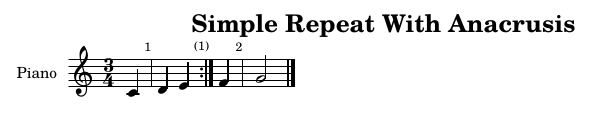
\includegraphics{SimpleRepeatWithAnacrusis.png}
\begin{lstlisting}[language=MusicXML]
<!-- ... ... ... ... ...-->
    <measure number="0" implicit="yes" width="144.60">
	  	<!-- ... ... ... ... ...-->
      <attributes>
        <divisions>1</divisions>
	  		<!-- ... ... ... ... ...-->
        </attributes>
      <note default-x="73.07" default-y="-50.00">
        <pitch>
          <step>C</step>
          <octave>4</octave>
          </pitch>
        <duration>1</duration>
        <voice>1</voice>
        <type>quarter</type>
        <stem>down</stem>
        </note>
      </measure>
<!--=========================================================-->
    <measure number="1" width="162.29">
      <note default-x="10.00" default-y="-45.00">
        <pitch>
          <step>D</step>
          <octave>4</octave>
          </pitch>
        <duration>1</duration>
        <voice>1</voice>
        <type>quarter</type>
        <stem>up</stem>
        </note>
      <note default-x="76.96" default-y="-40.00">
        <pitch>
          <step>E</step>
          <octave>4</octave>
          </pitch>
        <duration>1</duration>
        <voice>1</voice>
        <type>quarter</type>
        <stem>up</stem>
        </note>
      <barLine location="right">
        <bar-style>light-heavy</bar-style>
        <repeat direction="backward"/>
        </barLine>
      </measure>
<!--=========================================================-->
    <measure number="2" width="96.76">
      <note default-x="10.00" default-y="-35.00">
        <pitch>
          <step>F</step>
          <octave>4</octave>
          </pitch>
        <duration>1</duration>
        <voice>1</voice>
        <type>quarter</type>
        <stem>up</stem>
        </note>
      </measure>
<!--=========================================================-->
    <measure number="3" width="143.60">
      <note default-x="10.00" default-y="-30.00">
        <pitch>
          <step>G</step>
          <octave>4</octave>
          </pitch>
        <duration>2</duration>
        <voice>1</voice>
        <type>half</type>
        <stem>up</stem>
        </note>
      <barLine location="right">
        <bar-style>light-heavy</bar-style>
        </barLine>
      </measure>
\end{lstlisting}


% -------------------------------------------------------------------------
% -------------------------------------------------------------------------
\section{Lyrics}
\mylabel{lyrics}
% -------------------------------------------------------------------------
% -------------------------------------------------------------------------


% -------------------------------------------------------------------------
\subsection{The '{\tt <lyric>}' element}
% -------------------------------------------------------------------------

In \mxml\, the '{\tt <lyrics>}' elements are sub-elements of the '{\tt <note>}' elements. The definition is in \gitschemafile{note.mod}:
\begin{lstlisting}[language=MusicXML]
<!ELEMENT lyric
	((((syllabic?, text),
	   (elision?, syllabic?, text)*, extend?) |
	   extend | laughing | humming),
	  end-line?, end-paragraph?, %editorial;)>
<!ATTLIST lyric
    number NMTOKEN #IMPLIED
    name CDATA #IMPLIED
    %justify;
    %position;
    %placement;
    %color;
    %print-object;
    %time-only;
    %optional-unique-id;
>
\end{lstlisting}

\sep

In lyrics:

\begin{itemize}
\item 	word extensions are	represented using the '{\tt <extend>}' element;

\item	hyphenation is indicated by the '{\tt <syllabic>}' element, which can be '{\tt <single>}',
	'{\tt <begin>}', '{\tt <end>}', or '{\tt <middle>}'. These represent single-syllable
	words, word-beginning syllables, word-ending syllables,
	and mid-word syllables, respectively;

\item	multiple syllables on a single
	note are separated by '{\tt <elision>}' elements. A hyphen in the
	text element should only be used for an actual hyphenated
	word;

\item	two text elements that are not separated by an
	'{\tt <elision>}' element are part of the same syllable, but may have
	different text formatting.
\end{itemize}

\sep

The '{\tt <text>}' sub-element contains the text to be sung. It can have attributes controlling the way it is displayed:
\begin{lstlisting}[language=MusicXML]
<!ELEMENT text (#PCDATA)>
<!ATTLIST text
    %font;
    %color;
    %text-decoration;
    %text-rotation;
    %letter-spacing;
    xml:lang NMTOKEN #IMPLIED
    %text-direction;
>
<!ELEMENT syllabic (#PCDATA)>
\end{lstlisting}


\sep

For example, the first note of \gitmxmlfile{lyrics/QuemQueritis.xml} contains the single word '{\tt Quem}':\\
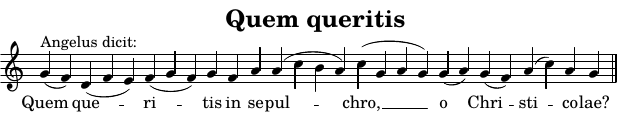
\includegraphics{QuemQueritis.png}
\begin{lstlisting}[language=MusicXML]
			<note>
				<pitch>
					<step>G</step>
					<octave>4</octave>
				</pitch>
				<duration>2</duration>
				<voice>1</voice>
				<type>quarter</type>
				<stem>up</stem>
				<notations>
					<slur type="start" number="1"/>
				</notations>
				<lyric number="1">
					<syllabic>single</syllabic>
					<text>Quem</text>
				</lyric>
			</note>
\end{lstlisting}


% -------------------------------------------------------------------------
\subsection{Stanzas}
% -------------------------------------------------------------------------

Stanzas are not represented in \mxml\ per se, but implicitly: the '{\tt number}' attribute of the '{\tt <lyric>}' element is used to specify the stanza number.

\sep

For example, in \gitmxmlfile{lyrics/MultipleStanzas.xml}, the first note (E\raisebox{0.35em}{$\flat$}) of the first chord in the upper staff contains the lyrics for the first syllable of all the successive stanzas, preceded by the stanza number and a dot:\\
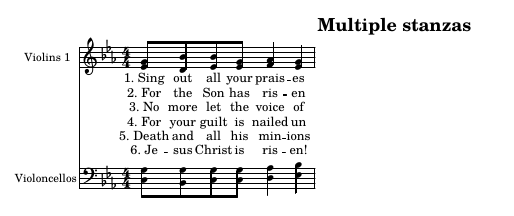
\includegraphics{MultipleStanzas.png}
\begin{lstlisting}[language=MusicXML,caption={Multiple stanzas example}]
      <note default-x="129.06" default-y="-40.00">
        <pitch>
          <step>E</step>
          <alter>-1</alter>
          <octave>4</octave>
          </pitch>
        <duration>1</duration>
        <voice>1</voice>
        <type>eighth</type>
        <stem>up</stem>
        <beam number="1">begin</beam>
        <lyric number="1">
          <syllabic>single</syllabic>
          <text>1. Sing</text>
          </lyric>
        <lyric number="2">
          <syllabic>single</syllabic>
          <text>2. For</text>
          </lyric>
        <lyric number="3">
          <syllabic>single</syllabic>
          <text>3. No</text>
          </lyric>
        <lyric number="4">
          <syllabic>single</syllabic>
          <text>4. For</text>
          </lyric>
        <lyric number="5">
          <syllabic>single</syllabic>
          <text>5. Death</text>
          </lyric>
        <lyric number="6">
          <syllabic>begin</syllabic>
          <text>6. Je</text>
          </lyric>
        </note>
      <note default-x="129.06" default-y="-30.00">
        <chord/>
        <pitch>
          <step>G</step>
          <octave>4</octave>
          </pitch>
        <duration>1</duration>
        <voice>1</voice>
        <type>eighth</type>
        <stem>up</stem>
        </note>
\end{lstlisting}


% -------------------------------------------------------------------------
% -------------------------------------------------------------------------
\section{Multiple voices}
\mylabel{multipleVoices}
% -------------------------------------------------------------------------
% -------------------------------------------------------------------------

Let's look in some detail at the score specified in \gitmxmlfile{multistaff/MultipleVoicesPerPart.xml}:\\
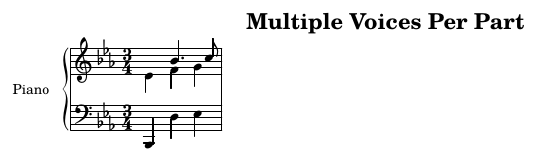
\includegraphics{MultipleVoicesPerPart.png}

\sep

The first voice in upper staff '{\tt 1}' has number '{\tt 1}'. The '{\tt <forward>}' element is used because there no note in this voice upon the first beat, whose duration is '{\tt 96}' divisions. This element allows \drawing\ to continue a bit further in the voice, without drawing rests in-between.:
\begin{lstlisting}[language=MusicXML]
      <forward>
        <duration>96</duration>
        <voice>1</voice>
        <staff>1</staff>
      </forward>
      <note default-x="154">
        <pitch>
          <step>B</step>
          <alter>-1</alter>
          <octave>4</octave>
        </pitch>
        <duration>144</duration>
        <voice>1</voice>
        <type>quarter</type>
        <dot/>
        <stem default-y="15.5">up</stem>
        <staff>1</staff>
      </note>
      <note default-x="225">
        <pitch>
          <step>C</step>
          <octave>5</octave>
        </pitch>
        <duration>48</duration>
        <voice>1</voice>
        <type>eighth</type>
        <stem default-y="18">up</stem>
        <staff>1</staff>
      </note>
\end{lstlisting}

\sep

The notes in voice '{\tt 2}' in staff '{\tt 1}' can now be described, but only after a '{\tt <backup>}' element that places the "\drawing\ position" back to the beginning of the measure:
\begin{lstlisting}[language=MusicXML]
      <backup>
        <duration>288</duration>
      </backup>
      <note default-x="108">
        <pitch>
          <step>D</step>
          <octave>4</octave>
        </pitch>
        <duration>96</duration>
        <voice>2</voice>
        <type>quarter</type>
        <stem default-y="0.5">up</stem>
        <staff>1</staff>
      </note>
      <note default-x="154">
        <pitch>
          <step>F</step>
          <octave>4</octave>
        </pitch>
        <duration>96</duration>
        <voice>2</voice>
        <type>quarter</type>
        <stem default-y="-63">down</stem>
        <staff>1</staff>
      </note>
      <note default-x="201">
        <pitch>
          <step>G</step>
          <octave>4</octave>
        </pitch>
        <duration>96</duration>
        <voice>2</voice>
        <type>quarter</type>
        <stem default-y="-60.5">down</stem>
        <staff>1</staff>
      </note>
\end{lstlisting}

\page

Then comes the specification of voice '{\tt 3}' in staff '{\tt 2}', again after a '{\tt <backup>}' element to place the \drawing\ position at the beginning of the measure:
\begin{lstlisting}[language=MusicXML]
      <backup>
        <duration>288</duration>
      </backup>
      <note default-x="108">
        <pitch>
          <step>B</step>
          <alter>-1</alter>
          <octave>1</octave>
        </pitch>
        <duration>96</duration>
        <voice>3</voice>
        <type>quarter</type>
        <stem default-y="5.5">up</stem>
        <staff>2</staff>
      </note>
      <note default-x="154">
        <pitch>
          <step>D</step>
          <octave>3</octave>
        </pitch>
        <duration>96</duration>
        <voice>3</voice>
        <type>quarter</type>
        <stem default-y="-55.5">down</stem>
        <staff>2</staff>
      </note>
      <note default-x="201">
        <pitch>
          <step>E</step>
          <alter>-1</alter>
          <octave>3</octave>
        </pitch>
        <duration>96</duration>
        <voice>3</voice>
        <type>quarter</type>
        <stem default-y="-50.5">down</stem>
        <staff>2</staff>
      </note>
\end{lstlisting}

% -------------------------------------------------------------------------
% -------------------------------------------------------------------------
\section{Creating MusicXML data}
% -------------------------------------------------------------------------
% -------------------------------------------------------------------------

This can be done in various ways:
\begin{itemize}
\item by hand, using a text editor: possible, but unrealistic for usual scores;
\item by exporting the score as an \mxml\ text file with a GUI music score editor;
\item by scanning a graphics files containing a ready-to-print score, with tools such as PhotoScore Ultimate\texttrademark;
\item by programming an application that outputs \mxml\ text.
\end{itemize}

This author has performed manual text editing on some of the samples supplied with \libmusicxml\ in order to perform tests and debug \xmlToLy, but this is a particular case.

\sep

Exporting to \mxml\ is probably the most frequent way, and there are applications that do a good job at that. If an application supports say strings instruments scordaturas in scores, then creating a '{\tt <scordatura>}' element is not very difficult.

\page

Scanning graphical scores is a tough problem:  how do you tell lyrics from annotations such as '{\tt cresc.}' or tempos such as '{\tt Allegro}'? One usually has to manually fix scanning errors and the category of some text fragments after scanning to get good results. And, of course, the scanning application should create quality \mxml\ data.

\sep

Creating \mxml\ by an application is a matter of computer programming, and requires software development skills. As an example, \libmusicxml\ supplies the necessary tools, and one can obtain:

\begin{lstlisting}[language=MusicXML]
       <attributes>
        <key>
          <fifths>-1</fifths>
          </key>
        </attributes>
\end{lstlisting}

with C++ code such as:

\begin{lstlisting}[language=CPlusPlus, caption={Creating a '{\tt <key>}' element in an application}]
  Sxmlelement attributes = factory::instance().create(k_attributes);

  Sxmlelement key = factory::instance().create(k_key);
  key->push (newElement(k_fifths, "1"));
  attributes->push (key);
\end{lstlisting}

\sep

Here is a score containing random 3-note chords created by \libmusicxmlSamples{RandomChords.cpp}, a C++ small program provided as a example of using \libmusicxml\ to create \mxml\ data:\\
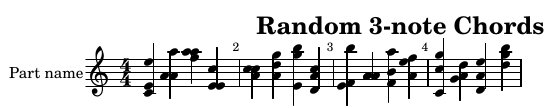
\includegraphics{RandomChords.png}


% -------------------------------------------------------------------------
% -------------------------------------------------------------------------
\section{Importing MusicXML data}
% -------------------------------------------------------------------------
% -------------------------------------------------------------------------

Many GUI applications provide a way to import \mxml\ data, often with some limitations. We show some of them below.

It is worth noting that \muse\ does a good job at issuing warnings if the \mxml\ data is not well-formed according to the DTD.


% -------------------------------------------------------------------------
\subsection{Small element, big effect}
% -------------------------------------------------------------------------

The '{\tt <harmony>}' element can contain an '{\tt <inversion>}' sub-element to indicate the number of the  chord inversion. Some applications ignore this element when importing \mxml\ data, because it takes  full knowledge of chords structures to compute the bass note of inverted chords.

\sep

Here is how \xmlToLy\ handlles the second inversion of the chord in \gitmxmlfile{harmonies/Inversion.xml}:\\
%\begin{figure}
%\caption{Harmony inversion from \gitmxmlfile{harmonies/Inversion.xml}}\mylabel{inversion}
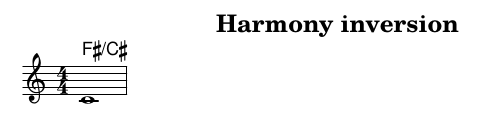
\includegraphics{Inversion.png}

\page

\begin{lstlisting}[language=MusicXML, caption={Harmony inversion}]
      <harmony>
        <root>
          <root-step>F</root-step>
          <root-alter>1</root-alter>
        </root>
        <kind>major</kind>
        <inversion>2</inversion>
      </harmony>
\end{lstlisting}
%\end{figure}


% -------------------------------------------------------------------------
\subsection{Elements handled in different ways}
% -------------------------------------------------------------------------

Multi-measure rests are specified in \mxml\ with the '{\tt <multiple-rest>}' element. All measures in the sequence have to be explicitly present in the \mxml\ data.

\sep

For example, the first two measures of \gitmxmlfile{rests/MultiMeasureRests.xml} are a multi-measure rest, described by:
\begin{lstlisting}[language=MusicXML]
  <part id="P1">
    <measure number="1">
      <attributes>
        <divisions>1</divisions>
        <key>
          <fifths>0</fifths>
          <mode>major</mode>
        </key>
        <time symbol="common">
          <beats>4</beats>
          <beat-type>4</beat-type>
        </time>
        <clef>
          <sign>G</sign>
          <line>2</line>
        </clef>
        <measure-style>
          <multiple-rest>2</multiple-rest>
        </measure-style>
      </attributes>
      <note>
        <rest/>
        <duration>4</duration>
        <voice>1</voice>
      </note>
    </measure>
    <!--=======================================================-->
    <measure number="2">
      <note>
        <rest/>
        <duration>4</duration>
        <voice>1</voice>
      </note>
    </measure>
    <!--=======================================================-->
\end{lstlisting}

\sep

This file is handled differently by various applications, as can be seen below.

\page

\muse\ displays it this way:\\
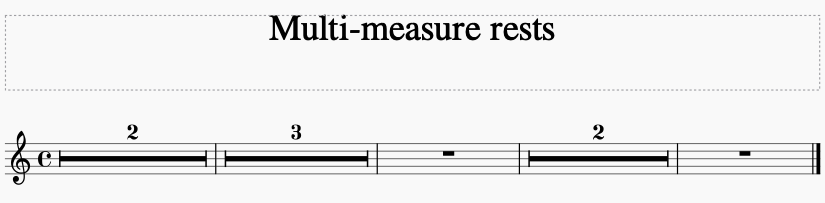
\includegraphics[scale=0.55]{MultiMeasureRestsMuseScore.png}

\sep \sep

\mxmlToLy\ produces:\\
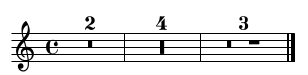
\includegraphics{MultiMeasureRestsMusicxml2ly.png}

\sep \sep

\sib\ produces:\\
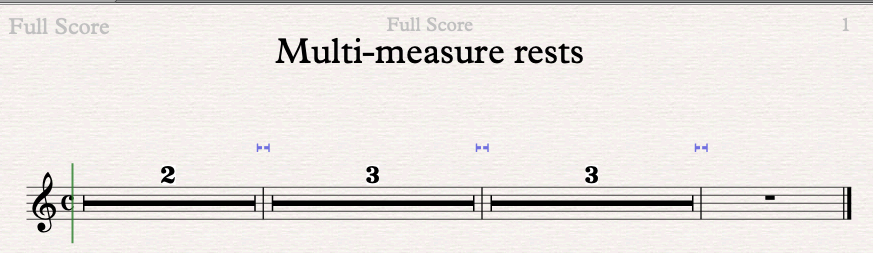
\includegraphics[scale=0.525]{MultiMeasureRestsSibelius.png}

\sep \sep

\fin\ produces:\\
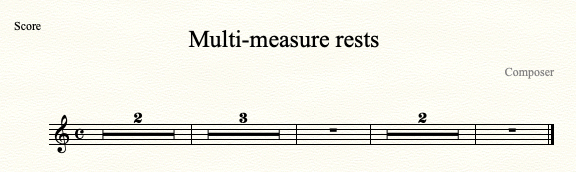
\includegraphics[scale=0.8]{MultiMeasureRestsFinale.png}

\sep \sep

\xmlToLy\ is still experimental, and currently produces:\\
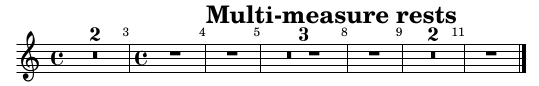
\includegraphics{MultiMeasureRestsXml2ly.png}

\page


% -------------------------------------------------------------------------
\subsection{Elements often not well handled}
% -------------------------------------------------------------------------

There are elements that are not displayed in a "standard" way by the usual music score editors. One of them is the '{\tt <beat-repeat>}', found for example in \gitmxmlfile{repeats/BeatRepeat.xml}.

\sep

\muse, \mxmlToLy, \xmlToLy\ and \sib\ produce the following, i.e. they ignore the beat repeat altogether:\\
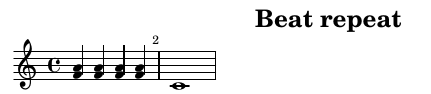
\includegraphics{BeatRepeatXml2ly.png}

\fin\ produces:\\
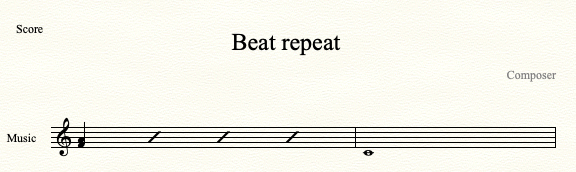
\includegraphics[scale=0.8]{BeatRepeatFinale.png}.

And if one exports that score from \fin\ to \mxml, the beat repeat information is lost, see \gitmxmlfile{repeats/BeatRepeatExportedFromFinale.xml}.


% -------------------------------------------------------------------------
\subsection{Elements usually not handled}
% -------------------------------------------------------------------------

There are elements that are not displayed by the usual music score editors, because there is no "standard" way to do so. One of them is the scordatura used on string instrument.

\sep

For example, the scordatura in \gitmxmlfile{strings/Scordatura.xml} is the case where the sixth string of the guitar is tuned a tone down to D, which can be described by:\\
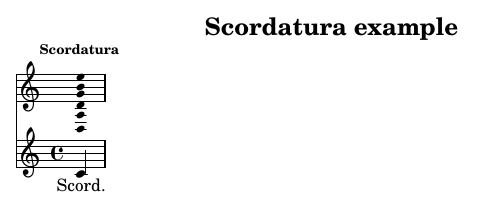
\includegraphics{Scordatura.png}

\begin{lstlisting}[language=MusicXML, caption={Scordatura example}]
          <scordatura>
              <accord std::string="6">
                <tuning-step>D</tuning-step>
                <tuning-alter>0</tuning-alter>
                <tuning-octave>3</tuning-octave>
              </accord>
              <accord std::string="5">
                <tuning-step>A</tuning-step>
                <tuning-alter>0</tuning-alter>
                <tuning-octave>3</tuning-octave>
              </accord>
              <accord std::string="4">
                <tuning-step>D</tuning-step>
                <tuning-alter>0</tuning-alter>
                <tuning-octave>4</tuning-octave>
              </accord>
              <accord std::string="3">
                <tuning-step>G</tuning-step>
                <tuning-alter>0</tuning-alter>
                <tuning-octave>4</tuning-octave>
              </accord>
              <accord std::string="2">
                <tuning-step>B</tuning-step>
                <tuning-alter>0</tuning-alter>
                <tuning-octave>4</tuning-octave>
              </accord>
              <accord std::string="1">
                <tuning-step>E</tuning-step>
                <tuning-alter>0</tuning-alter>
                <tuning-octave>5</tuning-octave>
              </accord>
          </scordatura>
\end{lstlisting}


% -------------------------------------------------------------------------
\subsection{A real challenge}
% -------------------------------------------------------------------------

The file \gitmxmlfile{challenging/BeethovenNinthSymphony.xml} is over 66 megabytes large -- it contains the whole score for this symphony.

\sep

The interested reader is urged to try and import this file into their favorite score editing sofware. This author's experience is that:
\begin{itemize}
\item \sib\ handles it alright;
\item \fin\ finds it well-formed, but too big to be opened;
\item \muse\ opens it, but then working on the file is extremely slow;
\item \mxmlToLy\ converts it to LilyPond\ syntax as of 2.19.83, and the result has some issues that should be fixed rather easily;
\item \xmlToLy\ converts it to LilyPond\ alright, but the issues in the \lcg\ show that this converter is still experimental\dots
\end{itemize}


% -------------------------------------------------------------------------
% -------------------------------------------------------------------------
\section{Conclusion}
% -------------------------------------------------------------------------
% -------------------------------------------------------------------------

\mxml\ supports other score elements such as harmonies and figured bass, as well as nested repeats. There is a lot of information about \mxml\ on the Internet. And of course, plenty of targeted, ready-to-use examples can be found in \gitsubdir{files/musicxml}.

\mxml\ has become a de facto standard for music scores data interchange between applications. The way it is exported and imported by the various applications is quite diverse though, and manual editing of the result is to be expected after import.

\sep

\mxml\ is not the whole story, though. The W3C Music Notation Community Group is working on MNX (\url{https://w3c.github.io/mnx}), as a successor to \mxml. One part of it is MNX-Common, which aims at being less verbose and more semantics-oriented than \mxml.

\sep

For example, consider:
\begin{lstlisting}[language=MusicXML]
<score-partwise version="3.1">
    <part-list>
        <score-part id="P1">
            <part-name>Music</part-name>
        </score-part>
    </part-list>
    <part id="P1">
        <measure number="1">
            <attributes>
                <divisions>1</divisions>
                <key>
                    <fifths>0</fifths>
                </key>
                <time>
                    <beats>4</beats>
                    <beat-type>4</beat-type>
                </time>
                <clef>
                    <sign>G</sign>
                    <line>2</line>
                </clef>
            </attributes>
            <note>
                <pitch>
                    <step>C</step>
                    <octave>4</octave>
                </pitch>
                <duration>4</duration>
                <type>whole</type>
            </note>
        </measure>
    </part>
</score-partwise>
\end{lstlisting}

\sep

In MNX-Common, this can be written in a more concise way:
\begin{lstlisting}[language=MusicXML,caption={MNX-Common example}]
<mnx>
    <score>
        <mnx-common profile="standard">
            <global>
                <measure>
                    <directions>
                        <time signature="4/4"/>
                    </directions>
                </measure>
            </global>
            <part>
                <part-name>Music</part-name>
                <measure barLine="regular">
                    <sequence>
                        <directions>
                            <clef sign="G" line="2"/>
                        </directions>
                        <event value="/1">
                            <note pitch="C4"/>
                        </event>
                    </sequence>
                </measure>
            </part>
        </mnx-common>
    </score>
</mnx>
\end{lstlisting}

Let's conclude with a tribute to the manual score engravers, whose skills have produced so many beautiful scores for centuries! Reaching the quality of their work is still a challenge for current music scoring software.


% -------------------------------------------------------------------------
% -------------------------------------------------------------------------
% postamble
% -------------------------------------------------------------------------
% -------------------------------------------------------------------------


% -------------------------------------------------------------------------
\end{document}
% -------------------------------------------------------------------------
